\documentclass[12pt]{article}
\usepackage{ctex}
\usepackage{graphicx}
\usepackage{indentfirst}
\usepackage{amsmath}
\usepackage{float}
\usepackage{amssymb}
\usepackage{bm}
\title{第九周作业报告}
\author{佐藤拓未 20300186002}
\date{}

\begin{document}
	
	\maketitle

\begin{center}
	\textbf{第一问}
\end{center}
\noindent 对方程(3.1.3), 如果边界条件改为$u(0)=0,\frac{{\rm d}u}{{\rm d}x}(1)+u(1)=0$, 求其精确解: 并用三点差分格式离散求解, 同时分析差分格式的精度.\\
\quad \\
\textbf{解:} 不妨固定$a=1$, 对下列方程进行离散化
\begin{align*}
	\begin{cases}
		&-\frac{{\rm d}^2u}{{\rm d}x^2}+b\frac{{\rm d}u}{{\rm d}x}+cu=1,\quad x\in(0,1)\\
		&u(0)=\frac{{\rm d}u}{{\rm d}x}(1)+u(1)=0
	\end{cases}
\end{align*}
\noindent 可以采用虚拟点法, 考虑如下近似
\begin{align*}
	\begin{cases}
		&u^{'}=\frac{1}{2h}(u(x_{N+1})-u(x_{N-1}))=-u_N\\
		&\frac{-u_{N+1}+2u_N-u_{N-1}}{h^2}+b\cdot\frac{u_{N+1}-u_{N-1}}{2h}+c\cdot u_N=1
	\end{cases}
\end{align*}
\noindent 整理可得$(c-b+\frac{2}{h^2}+\frac{2}{h})u_N-\frac{2}{h^2}u_{N-1}=1$, 且只需要修改矩阵最后一行即可.\\
\underline{当$b=c=0$时}: 可以知道方程($3.1.3$)的解形如$u(x)=-\frac{x^2}{2}+dx+e$, 并带入边值条件可知真解为$u(x)=-\frac{x^2}{2}+\frac{3x}{4}$. 在数值上令$N=10$可观测到数值解与精确解非常贴近, 如图1所示.
\begin{figure}[H]
	\centering
	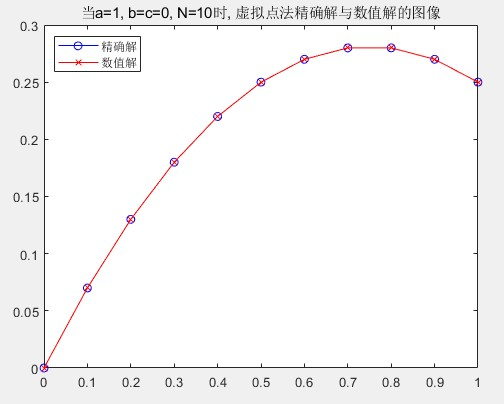
\includegraphics[width=1\textwidth]{13}
	\caption{当$a=1, b=c=0, N=10$时, 虚拟点法精确解与数值解的图像}
\end{figure}
\noindent 进一步讨论, 可令$h=2^{-n}$来观察其收敛阶, 可以看到此时虚拟点法并不会进一步降低精度, 如图2所示. 造成这样的原因可能是虚拟点法在前面几步就达到了机器精度.
\begin{figure}[H]
	\centering
	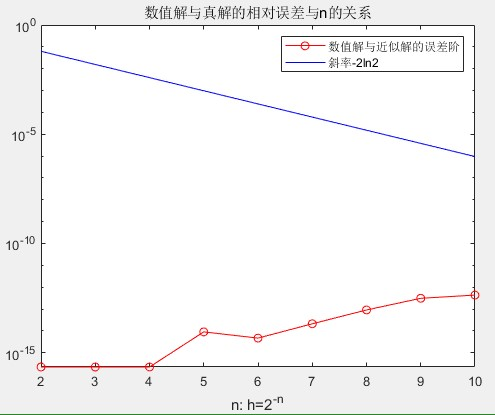
\includegraphics[width=1\textwidth]{14}
	\caption{当$a=1, b=c=0$时, 虚拟点法收敛阶}
\end{figure}
\noindent \underline{当$b,c$不为$0$}时: 可以知道真解为$$u(x)=\frac{1-e^{\lambda_1}(1+\lambda_1)}{c(e^{\lambda_1}(1+\lambda_1)-e^{\lambda_2}(1+\lambda_2))}e^{\lambda_2 x}-    \frac{1-e^{\lambda_2}(1+\lambda_2)}{c(e^{\lambda_1}(1+\lambda_1)-e^{\lambda_2}(1+\lambda_2))}e^{\lambda_1 x}+\frac{1}{c}$$
\noindent  其中$\lambda_{1,2}=-\frac{-b \pm \sqrt{b^2+4c}}{2}$, 不妨带入$b=-5,c=3$, 其收敛阶如图3所示.从图中可以看出, 数值解与真解的相对误差是二阶收敛的.
\begin{figure}[H]
	\centering
	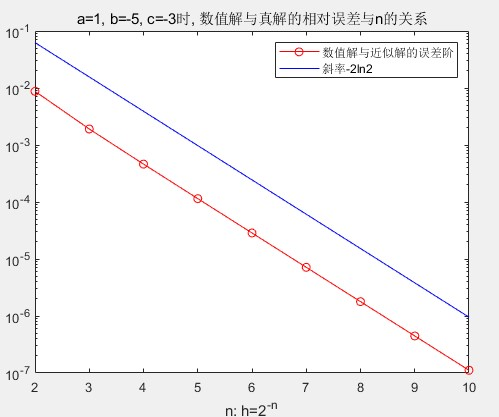
\includegraphics[width=1\textwidth]{15}
	\caption{当$a=1, b=-5,c=-3$时, 虚拟点法收敛阶}
\end{figure}
\noindent 综上所述, 当方程的情形非常简单时(例如, $b=c=0$), 虚拟点法求数值解的收敛速度是非常快的, 从而在前几步就达到了机器精度; 当$b,c$不为0时, 在前几步的精度并不能像前者一样直接达到机器精度, 但是随着步长$h$的减小, 数值解的相对误差呈现了二阶收敛.\\
\quad \\

\begin{center}
	\textbf{第二问}
\end{center}
\noindent 假设$u(x)$在区间$x\in(0,1)$满足:
\begin{align*}
	\frac{{\rm d}}{{\rm d}x}(a(x)\frac{{\rm d}u}{{\rm d}x})&=1,
\end{align*}
\noindent 且在端点$u(0)=u(1)=0$, 这里$a(x)$为分片常数:
\begin{align*}
	a(x)=\begin{cases}
		1,\quad &x\in(0,\frac{1}{2}),\\
		2,\quad &x\in(\frac{1}{2},1).
	\end{cases}
\end{align*}
\noindent 如果$u(x)$函数值和$a(x)\frac{{\rm d}u}{{\rm d}x}$在点$x=\frac{1}{2}$连续, 则证明
\begin{align*}
	u(x)=\begin{cases}
		\frac{1}{2}x^2-\frac{5}{12}x,&x\in(0,\frac{1}{2}),\\
		\frac{1}{4}x^2-\frac{5}{24}x-\frac{1}{24},\quad &x\in(\frac{1}{2},1).
	\end{cases}
\end{align*}
\noindent 并请用三点差分格式来求解这个问题: 考虑$h=2^{-n}$和$h=3^{-n}$的情况. 说明差分格式误差和网格的关系.\\
\quad \\
\textbf{解:} 分段求解这个问题, 首先由于$a(x)$是分段常数, 从而有以下
\begin{align*}
	u(x)=\begin{cases}
		\frac{x^2}{2}+bx+c,\quad x\in(0,\frac{1}{2})\\
		\frac{x^2}{4}+dx+e,\quad x\in(\frac{1}{2},1)
	\end{cases}
\end{align*}
\noindent 其中$b,c,d,e$均为常数, 代入$u(0)=u(1)=0$可得
\begin{align*}
	\begin{cases}
		c=0\\
		e=-(\frac{1}{4}+d)
	\end{cases}
\end{align*}
\noindent 再代入$u(\frac{1}{2}^-)=u(\frac{1}{2}^+)$以及$\frac{{\rm d}u}{{\rm d}x}\vert_{x=\frac{1}{2}^-}=2\frac{{\rm d}u}{{\rm d}x}\vert_{x=\frac{1}{2}^+}$, 则有
\begin{align*}
	\begin{cases}
		\frac{5}{16}+\frac{b}{2}=-\frac{d}{2}\\
		b=2d
	\end{cases}
\end{align*}
\noindent 从而解得
\begin{align*}
	\begin{cases}
		b=-\frac{5}{12}\\
		c=0\\
		d=-\frac{5}{24}\\
		e=-\frac{1}{24}
	\end{cases}
\end{align*}
\noindent 由此可得出真节具有题干中的分段形式, 且其图像如下所示, 可以发现真解在$x=\frac{1}{2}$时不具有连续导数.
\begin{figure}[H]
	\centering
	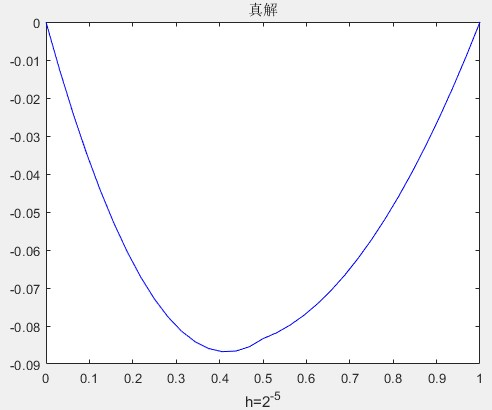
\includegraphics[width=0.71\textwidth]{8}
	\caption{第二问真解图像}
\end{figure}
\noindent 再考虑用三点差分格式求解原问题, 由于$a(x)$是分段常数, 从而要修改三点差分格式所对应的矩阵, 新的矩阵$A^{'}$为
\begin{align*}
	A^{'}=\frac{1}{h^2}\cdot\begin{pmatrix}
		 2 & -1\\
		 -1 & 2&-1\\
		&\ddots&\ddots &\ddots\\
		&&-1&2&-1\\
		& && -2&4&-2\\
		&&&&\ddots&\ddots&\ddots\\
		&&&&&-2&4&-2\\
		&&&&&&-2&4
	\end{pmatrix}
\end{align*}
\noindent \underline{当$h=3^{-n}$时}: 我们考虑不同步长$h=3^{-n}$下, 绝对误差的最大值与$n$的关系, 见图5. 可以发现绝对误差的最大值实际上是慢慢增大, 且绝对误差的最大值在$x_i=\frac{1}{2}$附近取到的, 见图6(以$h=3^{-8}$为例).
\begin{figure}[H]
	\centering
	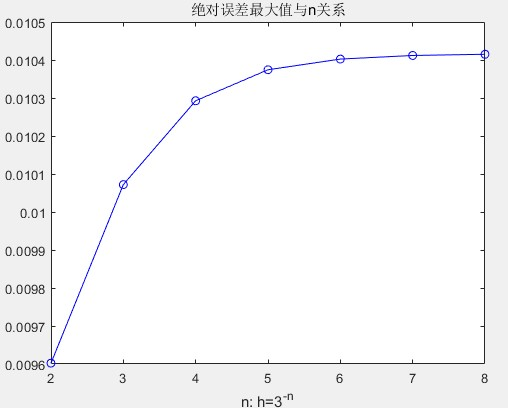
\includegraphics[width=0.7\textwidth]{9}
	\caption{当$h=3^{-n}$时, 绝对误差与$n$的关系}
\end{figure}
\begin{figure}[H]
	\centering
	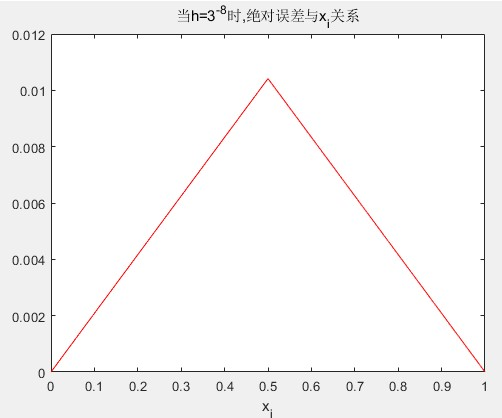
\includegraphics[width=0.71\textwidth]{10}
	\caption{当$h=3^{-8}$时, 近似解与真解在每点上的绝对误差}
\end{figure}
\noindent \underline{当$h=2^{-n}$时}: 用以上方法考虑绝对误差的最大值与$n$的关系, 见图7与8.
\begin{figure}[H]
	\centering
	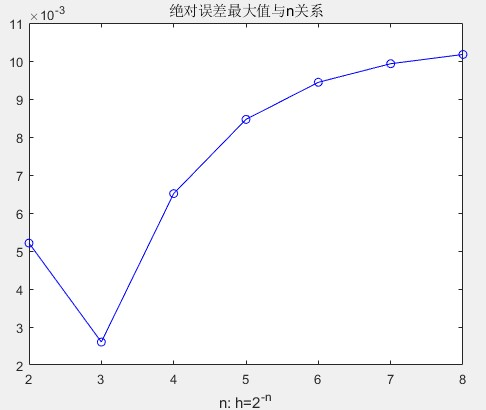
\includegraphics[width=0.65\textwidth]{11}
	\caption{当$h=2^{-n}$时, 绝对误差与$n$的关系}
\end{figure}

\begin{figure}[H]
	\centering
	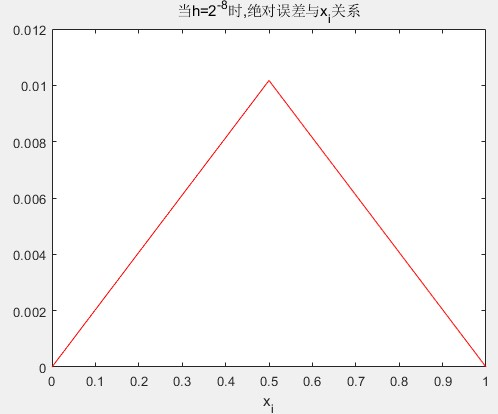
\includegraphics[width=0.63\textwidth]{12}
	\caption{当$h=2^{-8}$时, 近似解与真解在每点上的绝对误差}
\end{figure}
\noindent 造成以上原因有以下两方面: 1)矩阵$A^{'}$从中间行开始乘以常数, 且由于$A^{'}$并不是分块对称阵, 从而不能用分块求逆来求解数值解$\overset{\rightarrow}{u}$; 2)当$h=2^{-n}$或$3^{-n}$会随着$n$的增大而趋于0, 从而容易在数值上产生误差, 从而进一步导致数值解与真解的误差增大.\\
\quad \\

\begin{center}
	\textbf{第三问}
\end{center}
\noindent 证明不等式(3.1.54), 并用它来证明当$c(x)=0$时, 下述方程三点差分格式的收敛性:
\begin{align*}
	-\frac{{\rm d}^2u}{{\rm d}x^2}&=f(x),\quad u(0)=u(1)=0,
\end{align*}
\noindent 且三点差分格式函数值和导数值都是两阶收敛的.\\
\quad \\
\textbf{证明:} 考虑$-\delta_x^2u_i=\frac{-e_{i+1}+2e_i-e_{i-1}}{h^2}=f_i$, 其中$h=\frac{1}{N}$, $f_i=f(x_i)$. 同时, 由截断误差定义可知
\begin{align*}
	R_i&=-\delta_x^2u(x_i)-f_i\\
	&=\frac{-u(x_{i+1})+2u(x_i)-u(x_{i-1})}{h^2}+u^{''}(x_i)\\
	&=-\frac{h^2}{12}u^{(4)}(x_i)+O(h^4)
\end{align*}
\noindent 考虑$e_i=u(x_i)-u_i$, 则$-\delta_x^2e_i=R_i$, 且$e_0=e_N=0$. 记$\delta_x^+e_i=\frac{e_{i+1}-e_i}{h}$, 并考虑以下内积
\begin{align*}
	-\sum_{i=1}^{N-1}e_i\cdot\delta_x^2e_i&=-\frac{1}{h}\sum_{i=1}^{N-1}e_i(\delta_x^+e_i-\delta_x^+e_{i-1})\\
	&=\sum_{i=0}^{N-1}(\delta_x^+e_i)^2
\end{align*}
\noindent 再由Hölder不等式, 就有$$\vert \vert   \delta_x^+\overset{\rightarrow}{e_i } \vert  \vert^2_{l^2}=-\sum_{i=1}^{N-1}e_i\cdot\delta_x^2e_i=\sum_{i=1}^{N-1}R_i \cdot e_i\le \vert \vert \overset{\rightarrow}{R} \vert \vert_{l^2}\cdot \vert \vert   \overset{\rightarrow}{e}\vert \vert _{l^2}$$
\noindent 另一方面, 由$e_i=(e_i-e_{i-1})+\cdots+(e_1-e_0)=h\cdot\sum_{j=0}^{i-1}\delta_x^+e_j$, 可得$\vert \vert \overset{\rightarrow}{e}\vert \vert^2_{l^2}\le\frac{1}{2}\vert \vert \delta_x^2\overset{\rightarrow}{e_i } \vert  \vert^2_{l^2}$, 从而最终有不等式(3.1.54): $\vert \vert \overset{\rightarrow}{e}\vert \vert_{l^2}\le \vert \vert \overset{\rightarrow}{R} \vert \vert_{l^2}$. 故此时三点差分格式是收敛的, 且由于
\begin{align*}
	\vert \vert \overset{\rightarrow}{R} \vert \vert_{l^2}&=O(h^{\frac{3}{2}})\\
	\vert \vert \overset{\rightarrow}{e} \vert \vert_{l^2}&=O(h^{\frac{3}{2}})\\
	\frac{\vert \vert \overset{\rightarrow}{e}\vert \vert_{l^2}}{\vert \vert \overset{\rightarrow}{u} \vert \vert_{l^2}}&=O(h^2)
\end{align*}
\noindent 可知三点差分格式函数值是二阶收敛的. 再由式$\vert \vert   \delta_x^+\overset{\rightarrow}{e_i } \vert  \vert^2_{l^2}\le\vert \vert \overset{\rightarrow}{R} \vert \vert_{l^2}\cdot \vert \vert   \overset{\rightarrow}{e}\vert \vert _{l^2}$, 从而也有导函数值的二阶收敛性: $\frac{\vert \vert   \delta_x^+\overset{\rightarrow}{e_i } \vert  \vert_{l^2} }{\vert \vert \overset{\rightarrow}{u^{'}}\vert \vert_{l^2}}=O(h^2)$, 得证.\\
\quad \\
\textbf{注记:} 上述证明过程中用到了$\vert \vert \overset{\rightarrow}{u}\vert \vert_{l^2}, \vert \vert \overset{\rightarrow}{u^{'}}\vert \vert_{l^2}=O(h^{-\frac{1}{2}})$, 这是因为由数值积分复化梯形公式
\begin{align*}
	\int_{0}^{1}u(x)^2 {\rm d}x&=\sum_{i=0}^{N-1}\frac{h}{2}(u(x_i)^2+u(x_{i+1})^2)+O(h^2)\\
	&=h\vert \vert \overset{\rightarrow}{u} \vert \vert^2_{l^2}+O(h^2)
\end{align*}
而等式左边定积分为常数, 从而就有$\vert \vert \overset{\rightarrow}{u} \vert \vert_{l^2}=O(h^{-\frac{1}{2}})$, $u^{'}$的$l^2$范数同理.\\
\quad \\





\begin{center}
	\textbf{第四问}
\end{center}
\noindent 证明当$a(x)\ge \alpha >0$不是常数时, 对应问题:
\begin{align*}
	-\frac{{\rm d}}{{\rm d}x}(a(x)\frac{{\rm d}u}{{\rm d}x})&=f,
\end{align*}
\noindent 三点差分格式的极值原理仍然成立, 并给出三点差分格式的最大模误差估计.\\
\quad \\
\textbf{证明:} 先给出三点差分格式
\begin{align*}
	-\delta_{x}^2(\alpha_i u_i)&\overset{\triangle}{=}\alpha_i\frac{-u_{i+1}+2u_i-u_{i-1}}{h^2}-\frac{a_{i+1}-\alpha_{i-1}}{2h}\cdot\frac{u_{i+1}-u_{i-1}}{2h}\\
	&=\frac{-(\alpha_{i+1}+4\alpha_i-\alpha_{i-1})u_{i+1}+8\alpha_i u_i-(-\alpha_{i+1}+4\alpha_i+\alpha_{i-1})u_{i-1}}{4h^2}
\end{align*}
\noindent 如果当$\alpha_{i+1}+4\alpha_i-\alpha_{i-1}\ge0$, 那么$\alpha_{i+1}\le 4\alpha_i-\alpha_{i-1}$, 从而也有$-\alpha_{i+1}+4\alpha_i-\alpha_{i-1}\ge0$, 即三点差分格式中$u_{i+1}$与$u_{i-1}$前系数是同号的.\\
此时设$f_i\ge0$, 且$u_0=u_N=0$, 并且$u_i$($1\le i \ge N$), 且不妨$\alpha_{i+1}+4\alpha_i-\alpha_{i-1}\ge0$, 那么有以下
\begin{align*}
	(\alpha_{i+1}+4\alpha_i-\alpha_{i-1})u_{i+1}&=-4h^2 f_i+8\alpha_i u_i -(-\alpha_{i+1}+4\alpha_i+\alpha_{i-1})u_{i-1}\\
	&\le 8\alpha_i u_i -(-\alpha_{i+1}+4\alpha_i+\alpha_{i-1})u_{i-1}\\
	&\le  8\alpha_i u_i -(-\alpha_{i+1}+4\alpha_i+\alpha_{i-1})u_{i}\\
	&=(\alpha_{i+1}+4\alpha_i-\alpha_{i-1})u_{i}
\end{align*}
\noindent 再由$\alpha_{i+1}+4\alpha_i-\alpha_{i-1}$也大于等于$0$, 可推出$u_{i+1}\le u_i$, 从而$u_{i+1}$只能为最小值, 同理$u_{i-1}$也为最小值, 证毕.\\
\quad \\
\noindent 考虑最大模的误差估计: 记$e_i=u(x_i)-u_i$, 且$e_0=e_N=0$, 由于三点差分格式由两部分线性组成: 1)标准三点差分格式(2阶); 2)两个中心差商乘积(从而也是2阶), 故三点差分格式的局部截断误差$R_i=O(h^2)$, 考虑$	-\delta_{x}^2e_i=R_i$, 并且对$u(x)$有四阶导数有界控制(记为$M_4$), 以及对$\alpha(x)$有三阶导数有界控制(记为$M_3$)时, 由
\begin{align*}
	\begin{cases}
		&-\delta{x}^2 e_i =R_i\\
		&e_0=e_N=0
	\end{cases}
\end{align*}
\noindent 最终由比较原理可得: $\vert \vert \overset{\rightarrow}{e_i} \vert \vert_{l^{\infty}}\le CM_3M_4h^2 $.
\end{document}